\newenvironment{fenster}{%
  \begin{addmargin*}[
  5em]{5em}%
    \begin{minipage}{\linewidth}%
    \vspace{1em}
      \rule{\linewidth}{2pt}%
}{%
    \rule[
.25\baselineskip]{\linewidth}{2pt}%
\vspace{1em}
    \end{minipage}%
  \end{addmargin*}%
}
\renewcommand{\H}{\textsf{H}}
\renewcommand{\O}{\textsf{O}}
% /mnt/backup/safe-with-time/torben/safed/y2009/0411
\section{Fundamentals of fluorescence}
\begin{summary}
  Here we give a short overview of the field of fluorescence of
  molecules in order to introduce the terms Stokes' shift, triplet
  state and photobleaching.
\end{summary}
\subsection{Construction of molecular orbitals}
First we consider a very simple molecule: We move the nuclei of two
hydrogen atoms and move them slowly together. When the nuclei have a
big distance, the atoms exist as two separate entities without
influence on each other.
\begin{figure}[!hbt]
  \centering
  \input{flu-potential_my.eps_tex}
  \caption{Schematic electron density maps and potential curves for
    ground state $\H_2$ and excited state $\H_2^*$ of molecular
    hydrogen and the cation $\H_2^+$ of molecular hydrogen
    \citep[inspired from][p.~258]{Haken2006}.}
  \label{fig:flu-potential_my}
\end{figure}

For internuclear distances in between these two extremes, we express
molecular orbitals as a linear combination of atomic orbitals and
calculate their potential energy in dependence of the distance between
the nuclei (see \figref{fig:flu-potential_my}). The curve for
$\sigma_g\sigma_g^1\Sigma_g^+$ is minimal at a internuclear distance
$R$ of approximately 1.3 Bohr radii
($a_H=\unit[0.529\cdot10^{-8}]{cm}$). The compound of two protons and
two electrons is particularly stable for this distance. We call it the
hydrogen molecule $\H_2$.

Likewise a linear combination of the atomic orbitals of a ground state
hydrogen atom $\H$ with an excited hydrogen atom $\H^*$ lead to the
molecular orbital $\sigma_g\pi_u^1\Pi_u$. There, a minimum in the
potential occurs at an increased internuclear distance (bond
length). The excited atomic orbital has a reduced probability density
close to the nucleus but similar electron--electron
repulsion. Therefore the strength of the molecular bond (order of the
bond) is reduced.
\newcommand{\vmu}{\mbox{\boldmath{$\mu$}}}
\subsection{Absorption and emission of light}
A transition between a ground state $S_0$ to an excited state $S_1$
occurs, when a radiation field connects the two states. The connection
is described by the transition dipole moment
$\vmu_{0\rightarrow 1}$.
\begin{align}
  \vmu_{0\rightarrow 1} &= \int \psi^*_0 \vmu \psi_1 \textrm{d}^3\r
\end{align}
where $\psi_0$ and $\psi_1$ are wavefunctions for the ground and
excited state, respectively \citep{Klessinger1989}.

An incident photon can electronically excite a molecule from the
highest occupied molecular orbital (HOMO), usually the singlet ground
state $S_0$, into the lowest unoccupied molecular orbital (LUMO), the
singlet excited state $S_1$.\nomenclature{HOMO}{highest occupied
  molecular orbital}\nomenclature{LUMO}{lowest unoccupied molecular
  orbital} For this, the energy $E_\textrm{ph}=hc/\lambda$ of the
photon has to match the energy gap $\Delta E=E_{S_1}-E_{S_0}$ of a
possible electronic transition within the molecule (Bohr's frequency
condition).

Photons with wavelengths below \unit[200]{nm} have sufficient energy
to ionize molecules. On the other side of the spectrum, a dye that
absorbs in the near-infrared ($\unit[>700]{nm}$) has a low-lying
excited singlet state $S_1$ and potentially increased reactivity
\citep{Sauer2011}. Hence, most known stable and bright fluorophores
absorb and emit in the wavelength range between \unit[300]{nm} and
\unit[700]{nm}.

As opposed to atomic spectra the absorption bands of organic dyes
usually span several tens of nanometers\footnote{Note that wavelength
  isn't a convenient unit to characterize absorption bands. Rather one
  should use energy or wavenumbers.}. This is because dye molecules
are composed of many atoms and this structure can vibrate, rotate and
interact with the solvent.
\subsection{Vibration of molecules}
The distance between the two nuclei of the hydrogen molecule is not
rigid. The nuclei can oscillate around their position of equilibrium
at quantized frequencies. The vibration frequencies depend on the
order of the bond and the mass of the two nuclei. When a molecule is
electronically excited, its vibration frequencies decrease.
\begin{figure}[!hbt]
  \centering
  % (423-120)/423*7 = 4.77 ,trim=0 0 135 0,clip
  \input{flu-condon_my.eps_tex}
  \caption{Illustration of the Franck-Condon principle. Potential
    curves for either the same bond length in the
    excited state ({\bf left}) or a larger bond length in the
    excited state ({\bf right}). Electronic transition occurs
    instantaneously and excites higher vibro-rotational states in the
    right diagram. \citep[inspired from][p.~276]{Haken2006}.}
  \label{fig:flu-condon}
\end{figure}

\figref{fig:flu-condon} schematically shows potential curves for the
ground state $S_0$ and the first excited state $S_1$ of two different
molecules. The left graph depicts a molecule where the internuclear
distance is the same in the ground $S_0$ and excited $S_1$ stage. When
such a molecule absorbs a photon, its electron is excited but its
vibrational mode does not change. The anthracene molecule shows such
behaviour.

The right graph depicts a molecule that has a larger internuclear
distance in its excited state. When a photon is absorbed, the
electronic state of the molecule transitions into the higher state
$S_1$. The mass of the electron is much smaller than the
nucleus. Therefore the electronic transition takes place in a
timescale of $\unit[\sim10^{-15}]{s}$. In this duration the nuclei do
not move (\emph{Born-Oppenheimer approximation}: electronic
transitions occur as if the nuclei were fixed in place). The changed
bond length with the new orbital of the excited state $S_1$ drives the
nuclei into movement (excitation of vibro-rotational modes,
\emph{Franck-Condon principle}: electronic transition most likely
occurs without changes to the position of the nuclei and the intensity
of a vibrational transition depends on the overlap between the
vibrational wavefunctions).

\subsection{Depopulation pathways of excited states}
\begin{figure}[!hbt]
  \centering
  \def\svgscale{.8}
  {\small
  \input{flu-level_my.eps_tex}}
  \caption{A typical energy level diagram. The boxes depict orbitals,
    up and down arrows symbolize the spin of the outer electrons. Fat
    lines represent electronic states. Thinner lines indicate
    vibro-rotational states. Various processes are shown with their
    typical time scales. VR = vibro-rotational relaxation, ISC =
    intersystem crossing, IC = internal conversion \cite[inspired
    from][]{Haken2006}.}
  \label{fig:flu-level}
\end{figure}
The Jablonski diagram in \figref{fig:flu-level} summarizes information
about the energy levels of a molecule and possible transition
processes. If a molecule is in the ground state $S_0$ one of its outer
electrons can be excited by absorbing a photon to the first excited
singlet state $S_1$.  If the photon has an even higher energy, the
electron will go into the second excited singlet state $S_2$.

Transition from the ground state into higher electronic states than
$S_2$ is not usual in commonly used fluorophores and wavelength range.
Absorption of one photon doesn't change the spin of an electron and
therefore the transition $S_0\rightarrow T_1$ into the triplet state
$T_1$ only occurs with very low probability.

\subsubsection{Kasha's rule}
As described above, electronic excitation in general also leads to the
excitation of a vibro-rotational nonequilibrium state (Franck-Condon
state). In microscopy, fluorophores are often in solution, where they
experience at least $10^{12}$ collisions per second. Inter- and
intramolecular interactions bring the vibrations of the fluorophore
molecule back to thermal equilibrium\footnote{Rotation states have
  energies corresponding up to \unit[100]{$cm^{-1}$} (microwave),
  vibration states have energies corresponding to wavenumbers from 300
  to \unit[3000]{$cm^{-1}$} (infrared). Electronic states have
  energies in the visible. The number of excited molecules in thermal
  equilibrium is governed by the Boltzmann law and proportional to
  $\exp(-\Delta E/(k_BT))$. Therefore, at room temperature ($k_B
  T\sim\unit[200]{cm^{-1}}$), only rotation states are excited. } in a
very short timescale ($\unit[10^{-12}]{s}$). This is considerably less
then the lifetime of the electronic excitation (few
nanoseconds). Therefore spontaneous emission of a photon will occur
from the vibrational ground state $S_{1,v_1=0}$ (\emph{Kasha's rule}).

\subsubsection{Stokes' shift}
During emission of a fluorescence photon a Franck-Condon state of the
singlet ground state $S_0$ is excited and returns into thermal
equilibrium by vibro-rotational relaxation. Thus, some of the energy
of the original excitation photon is lost as heat. The emitted
fluorescence photon is red shifted compared to the excitation
photon. Technically the \emph{Stokes' shift} is defined as the
difference of the wavenumbers of the fluorescence maximum and
absorption maximum\footnote{Sometimes the Stokes' shift is also defined
  as the distance of the absorption maximum to the point where the
  normalized absorption and corrected fluorescence emission curves intersect.}.

In terms of wavelength the Stokes' shift usually corresponds a change
of 15 to \unit[30]{nm}. The Stokes' shift is bigger, when the shape and
position of the potential of the excited state $S_1$ differs from the
ground state $S1$ (see \figref{fig:flu-condon}, right). There are
fluorophores with more than \unit[100]{nm} Stokes shift.

\subsubsection{Internal conversion}
Often the transition $S_2\rightarrow S_1$ occurs by \emph{internal
  conversion} (IC) followed by vibro-rotational relaxation. During IC,
the electronic state transitions into a high vibro-rotational
excitation of a lower electronic state. The probability for IC is high
for a high density of vibrational target states.
% FIXME translate Zustandsdichte

For floppy, non-rigid molecules, IC is a competing process to
fluorescence $S_1\rightarrow S_0$. In dyes that absorb in the near
infrared, the energy gap between $S_0$ and $S_1$ is so small and the
vibrational states of highest energy of the singlet ground state $S_0$
(vibration of hydrogen bonds directly attached to the chromophore) are
close to $S_1$. This seriously reduces the efficiency of infrared dyes
\citep[p.~43]{Sauer2011}.


\subsubsection{Fluorescence quantum yield}
The \emph{fluorescence quantum yield} $\eta$ of a fluorophore is
defined as the quotient of the number of emitted (fluorescence)
photons and the number of absorbed photons. In dyes like rhodamine~6G
(in ethanol $\eta=0.94$ \cite{Fischer1996}) or anthracene
(9,10-diphenyl anthracene in cyclohexane $\eta=0.90$ \cite{Hamai1983})
its value can be nearly 1 in an appropriate solvent.


\subsubsection{Intersystem crossing}
There is a small probability that the HOMO electron doesn't relax by
internal conversion or emission of a fluorescence photon. Instead it
flips its spin (due to spin-orbit coupling\footnote{The probability of
  a spin flip is increased if heavier atoms are part of the
  molecule. E.g.\ while fluorescein has a triplet yield of 0.03, the
  triplet yield of eosin, a fluorescein derivative with four bromine
  substituents is 0.76 \citep[p.~37]{Sauer2011}.}). This process is
called \emph{intersystem crossing} and populates the first triplet
state $T_1$. A transition into the ground state $S_0$ would need
another spin-flip of the electron and is quite improbable. Therefore
the triplet state has a long lifetime (up to several seconds). The
radiative decay is called phosphorescence.
  

\subsection{Photobleaching and phototoxicity}
The prolonged lifetime of the triplet state $T_1$ increases the
probability for the excited molecule to collide with a partner and
react.

\begin{figure}[!hbt]
  \centering
  \input{oxygen.eps_tex}
  \caption{{\bf left:} Molecular orbitals of the oxygen molecule. {\bf
      right:} Molecular oxygen has the lowest energy in its triplet
    state ${}^3\Sigma$. Then the spins of the two $\pi^*-$electrons
    are parallel. Inspired from \citet{Linde2011a}.}
  \label{fig:oxygen}
\end{figure}


The ground state of the oxygen molecule is a triplet state ${}^3\O_2$,
with two unpaired electrons of parallel spin in its
$\pi^*-$orbitals\footnote{The antibonding molecular orbital $\pi^*$ of
  molecular oxygen is constructed by linear combination of two atomic
  orbitals of oxygen.}  (see \figref{fig:oxygen}). The triplet ground
state and its abundance in typical microscope samples are the reasons
why oxygen is so important when it comes to phototoxicity. If an
oxygen molecule comes into physical contact with a $T_1$ fluorophore,
e.g.\ ${}^3\textsf{Chlorophyll}^*$, the energy of the dye can be
transferred to the oxygen by an electron exchange energy transfer
mechanism in which the orbitals directly interact with each other
\citetext{\citealp[p.~438]{Haken2006} and \citealp{Linde2011a}}:
\begin{align}
  {}^3\O_2 + {}^3\textsf{Chlorophyll}^* \rightarrow
  {}^1\O^*_2+{}^1\textsf{Chlorophyll}
\end{align}
This reaction is also known as triplet--triplet annihilation.  There
are two forms of singlet oxygen, that form in competition: The lower
energy ${}^1\Delta$ and the short-lived, higher energy ${}^1\Sigma$
form ($T_{1/2}\sim\unit[10^{-9}]{s}$), with spin orientations as
depicted on the right of \figref{fig:oxygen}. During the transition
${}^1\Sigma\rightarrow{}^1\Delta$ an infra-red photon with
\unit[1268]{nm} wavelength is emitted \citep[p.~20]{Linde2011a}.

The resulting singlet oxygen ${}^1\Delta$ is very reactive. In a
typical specimen it diffuses only a few tens of nanometre until it
reacts with another molecule \citep{Sauer2011}. When it reacts with
the fluorophore, it can destroy it (photobleaching) also the singlet
oxygen can damage the DNA of living creatures. Plants have developed
several protection mechanisms against being exposed to too much
light. Within the cells they reorient and shift their chloroplasts in
order to expose them to less light \citep{Reshak2009}.  However, they
even have a molecular protection mechanism: They transfer the energy
of the chlorophyll onto carotenoid molecules and can prevent the
hazardous \emph{phototoxicity} effects of singlet oxygen
\citep{Krieger-Liszkay2005}.

Nowadays many methods are known to reduce photobleaching. Substitute
oxygen with noble gases or remove it enzymatically
\citep[p.~89]{Sauer2011}. Depopulate the triplet state by adding
reducing as well as oxidizing agents to the solvent
\citep{Vogelsang2008} or couple a triplet quencher directly to the
fluorophore \citep[p.~19]{Sauer2011}. For fixed samples it helps to
change the solvent or polymer.

In living specimen these techniques may reduce photobleaching, but
they can also have an effect on the biological system itself. Removing
oxygen will quite certainly have a negative effect. In order to reduce
phototoxicity it makes sense to think about the light management in
the microscope.


\section{Conventional microscopes}
\begin{summary}
  Microscopes that are in common use today do not optimally excite
  fluorophores within the specimen. In this section we outline how
  these microscopes work. We explain how out-of-focus blur severely
  limits the performance of the wide field microscope. Then we discuss
  how confocal microscopy improves the sectioning capability at the
  cost of increasing the phototoxic load on the specimen.
\end{summary}
The basic building block of microscopes are lenses. A lens is a piece
of glass with two polished spherical surfaces. Aspherical lenses also
exist but are much harder to manufacture because of their lower
symmetry. Light is slower in glass than in air. The shape of a lens
redirects photons and the thickness of the material can delay them. A
lens ideally focuses a parallel beam of light into a spot on its focal
plane. The distance between focal plane and the region where the rays
start to converge is called focal length and denoted by $f$.
\begin{figure}[!hbt]
  \centering
  \input{widefield-microscope.eps_tex}
  \caption{{\bf a)} Schematic of a modern microscope. The sample is in
    the front focal plane of the objective. The detection tube lens
    TL1 forms a magnified image on the camera. {\bf b)} Parallel laser
    epifluorescence excitation. The excitation tube lens focuses a
    laser into the back focal plane (BFP). The beam is reflected by a
    dichroitic beam splitter (BS) towards the objective. An extended
    area in the specimen is illuminated. Fluorescence light of lower
    wavelength returns through the objective, is transmitted through
    BS and forms an image on the camera. {\bf c)} Confocal
    microscope. A pinhole PH2 is imaged as a diffraction limited spot
    into the specimen. Returning fluorescence light is only detected
    when it passes through an aligned pinhole PH1. This configuration
    rejects light that doesn't originate from the front focal plane
    (green) of the objective.}
  \label{fig:widefield-microscope}
\end{figure}

The uncoloured beam in \figref{fig:widefield-microscope}~a) represents
rays that start from the intersection $O$ of the optical axis and the
front focal plane of the objective. The objective collects the rays
and collimates them into a beam that is parallel to the optical
axis. After traversing the tube length $f+f_\textrm{TL}$, the rays are
focused by the detection tube lens TL1 on the intersection $O'$ of its
focal plane and the optical axis. 

The blue beam corresponds to rays that start from an off-axis point
$P$ in the front focal plane of the objective. Behind the objective
the blue beam is a parallel beam. However, the beam is tilted relative
to the optical axis. The tube lens TL1 focuses the blue beam into a
spot at $P'$ on its focal plane.

The objective fulfils the Abbe sine condition -- it is aplanatic. The
microscope forms stigmatic\footnote{An imaging system collects some of
  the rays, that leave an object and directs them towards the
  image. If all rays that leave an object point converge in the
  conjugate image point, then we call the image point stigmatic.}
images of points from the front focal plane in the plane perpendicular
to the optical axis, containing $O'$ and $P'$. The plane with the
images is called intermediate image plane. It is magnified by the
factor $M$:
\begin{align}
  M=\frac{\overline{O'P'}}{\overline{OP}}=\frac{f_\textrm{TL}}{f}.
\end{align}
In our microscope we use an objective with magnification $M=63$. The
focal length of the tube lens is \unit[164.5]{mm} for most Zeiss
microscopes. Therefore the focal length of our objective is
$f=\unit[2.61]{mm}$.

Let's assume we have an opaque sample with just two small
($\diameter<\unit[120]{nm}$) holes with $\unit[2]{\mu m}$ distance
between them.  We put this object into the front focal plane of the
objective and position a camera on $O'$. When illuminating the mirror
from the side opposite to the objective, the camera will show two
spots with $\unit[126]{\mu m}$ distance.

\nomenclature{NA}{numerical aperture}

Note that \figref{fig:widefield-microscope} depicts a \emph{thin-lens
  model of a high numerical aperture objective} that fulfils Abbe's
sine condition. A real objective contains in the order of ten coated
lenses of different glass and crystalline materials. Their curvatures,
positions and materials were all carefully chosen, taking into account
manufacturing tolerances and wavelengths, so that the microscope
behaves as the thin-lens model predicts. Diffraction at the periphery
of the pupil in the back focal plane dictates the resolution, one can
achieve inside of the sample.

It is quite possible that heating to \unit[37]{${}^\circ$C} will ruin
such a high-precision instrument. A related source of aberrations
(departure of design performance) is the refractive index inside of
the specimen. In Appendix~\ref{sec:ray-aberration} we describe a more
complicated model that can predict the effect of embedding the sample
in water (instead of immersion oil with the same refractive index as
the glass).

\subsection{Widefield epifluorescence microscope}
Fluorescence photons are emitted in all directions, independent of the
original illumination direction. Therefore it is possible and
convenient to use the objective for excitation as well as
detection. This mode of microscopy is called epifluorescence (Greek:
$\varepsilon\pi\iota$; on, above).  In this configuration usually only
a small percentage of the excitation light returns due to diffraction
or reflection. This simplifies the separation of fluorescence light
from excitation light.  Furthermore parts of opaque specimen can be
imaged and it is beneficial that the illumination needs to be aligned
only once.

\nomenclature{BFP}{Back focal plane}

The red beam in \figref{fig:widefield-microscope}~b) is a parallel
laser. The excitation tube lens TL2 focuses the beam into the back
focal plane (BFP) of the objective. The beam is reflected at a
dichroitic beam splitter (BS). This is a glass plate that has been
coated with dielectric layers. The refractive index, thickness and
sequence of the layers are designed so that the excitation light is
reflected towards the objective. Excitation light, that is scattered
or reflected in the sample and returns through the objective is
reflected towards the light source. However, lower energy fluorescence
light returning from the objective is transmitted towards the
camera. Behind the objective the beam is parallel and illuminates the
specimen. The field of view is the demagnified diameter of the laser
beam before TL2.
\subsubsection*{Non-uniformity due to coherent interference}
Note that tiny dirt particles and coherent interference in laser beams
can produce unwanted non-uniformities in the illumination. As a remedy
the spatial coherence of the laser is sometimes reduced.  Incoherent
light emitting diodes, mercury or xenon arc lamps are often used
instead of lasers. In the latter case a band pass filter selects the
useful part of the spectrum of the excitation lamp upstream of the
dichroitic beam splitter.

\subsubsection{Out-of-focus blur}
However, independent of the choice of the light source, the wide field
microscope in epifluorescence configuration exposes many layers of the
sample. This leads to fluorescence of out-of-focus fluorophores.

There are two reasons, why out-of-focus fluorophores give blurred
images. Not even an ideal imaging system -- a device that forms
%% FIXME refer to maxwell or born/wolf
stigmatic images of all the points in one volume in another volume --
would form sharp images on the camera plane. After all, the camera is
just a plane and the object under observation is three dimensional.

Furthermore a microscope is far from being an ideal imaging system. In
a microscope it is not possible to obtain a sharp image of a different
slice of the object by changing the axial position of the camera
behind the tube lens TL1 \citep{Botcherby2007,Botcherby2008a}.
\subsubsection*{Deconvolution}
When a stack of several slices of an object is obtained, it is
possible to suppress the blurred part of each image in all the
others. These algorithms (deconvolution) can improve the perceived
quality of images in some stacks. However, there are two fundamental
problems:

First the \emph{missing cone problem} prevents focusing on a
homogeneous fluorescent plane. Physics dictates that there is always a
gap in the transfer function of the objective when the fluorescence
process is linear and the objective collects only photons from one
half space (see \figref{fig:missing-cone}). Not all spatial
frequencies within the transfer function attenuate with defocus
\citep{Neil1997}.

\begin{figure}[!hbt]
  \centering
  \input{missing-cone.eps_tex}
  \caption{Schematic depicting $k_xk_z-$cross sections of the support
    of optical transfer function (see Appendix~\ref{sec:app_hilo}) for
    microscope objectives with different collection angles. {\bf
      left:} Objectives, that only collect light that is directed into
    one half space, have the missing cone problem. There, low spatial
    frequencies don't attenuate with defocus. {\bf right:} Theoretical
    objective with larger collection angle and no missing cone.}
  \label{fig:missing-cone}
\end{figure}

Second, even with ideal detectors there is photon shot noise in the
image. In deconvolution algorithms the image of one slice is improved
by subtracting blurred versions of the other slices. When the blurred
intensity is large, its shot noise is high as well. Subtraction only
increases noise and a faint in-focus image can be severely
deteriorated by the noise of the out-of-focus light.
\subsection{Confocal microscope}
One way of addressing both problems of the wide field microscope is
depicted in \figref{fig:widefield-microscope}~c). In the confocal
microscope the whole field of view isn't illuminated simultaneously.
The excitation tube lens TL2 collimates the light coming from a
pinhole PH2 and illuminates the full back focal plane of the
objective. In the front focal plane of the objective the red beam then
converges to illuminate the smallest possible single spot. The spot
size is defined by diffraction at periphery of the BFP. However,
out-of-focus fluorophores are still being excited by the hour-glass
shaped illumination.

The eponymous idea of the confocal microscope is to replace the camera
with a pinhole PH1. This pinhole, if aligned carefully to the position
of the image of the focused laser spot, has no influence on the light
detected from in-focus fluorophores. However, an out-of-focus
fluorophore that is defocused by $\Delta z$ towards the objective will
lead to a diverging beam (colorless) at the tube lens and will be
imaged into a point behind the focal plane of the tube lens. The
pinhole only transmits a part of the circle of confusion. Hence
defocused fluorophores contribute less to the sensor signal.

An image of the in-focus specimen is obtained by scanning the pinholes
PH1 and PH2 over the field of view and measuring intensity at each
position individually. The optical removal of out-of-focus light
prevents degradation of the signal by its shot noise and improves the
point-spread function of the objective. The missing cone problem is
fixed and the resolution improved by a factor of two. Note however,
that information about out-of-focus fluorophores is lost which would
be obtained in a wide field microscope with deconvolution. Therefore a
wide field microscope will give better results when a lot is known
about the sample structure and this knowledge is fed into the
deconvolution. E.g.\ the localization of sparse beads of specific size
will be better in a wide field microscope.

The confocal microscope was invented in 1955 \todo{check patent
  citation} \citep{Minsky1961,Minsky1988} to reduce the influence of
scattering effects in neuron samples stained by Golgi's method. This
invention preceded the laser and was unfortunately not put into
practical use for biology until three decades later \citep{Amos1987}.
\subsection{Phototoxicity in conventional microscopes}
When imaging living specimen we should distinguish between useful and
unnecessary excitation. Taking into account the detection capabilities
of objective lenses we should maximize the ratio of in-focus to
out-of-focus fluorescence. The epifluorescent wide field and confocal
microscope surely do not represent an optimum in this regard.

The following chapter \ref{sec:approaches} will introduce other
microscopy techniques that are more considerate of where to deposit
excitation power within the specimen.
\subsection{2-photon laser scanning fluorescence microscopy}
If the laser intensity in the focal spot of a confocal microscope is
sufficiently high, then two infrared photons can be absorbed within
\unit[$\sim 5$]{fs} and excite the same electronic state.

In this regime, the fluorescence emission increases quadratically with
laser intensity. This non-linearity confines the excitation volume to
the vincinity of the focal plane \citep{Denk1990}. Fluorophores
outside of this region are not excited. Therefore this method produces
sectioned images by default and there is no need for a detection
pinhole.

As an additional benefit infrared light is scattered less than visible
light of half the wavelength. This increases penetration depth and
image quality. Photodamage outside of the focal volume is unlikely and
phototoxicity is much lower, compared to the single-photon confocal
microscope, when $z-$stacks are acquired.

However, the phototoxicity within the focal volume is higher and
techniques like ultramicroskopy (section
\ref{sec:light-sheet-microscopy}) with single-photon excitation are
preferable, when low overall phototoxicity is a requirement.

\section{Image detectors in wide field microscopy}
\label{sec:ccd-intro}
\begin{summary}
  Here we describe CCD\nomenclature{CCD}{charge-coupled devices}
  sensors and their characteristics.
\end{summary}
Charge-coupled devices are semiconductor devices that contain a 2D
grid of capacitors, formed by at least three groups of electrodes
(phases). Cycling the voltage on these electrodes allows to push
charges, which has been accumulated under the capacitors (registers)
into their neighbours. They turned out to be the ideal tool to move
charges, produced by photon absorption in light sensitive diodes,
across the substrate into read out logic.

Forty years of development lead to imaging devices with remarkable
charge transfer efficiency, high quantum efficiency (up to 95\% with
back illumination) and very low dark currents. Until ten years ago the
performance of CCD imagers in the low light regime was limited by the
noise of the read out amplifier (a few electrons per pixel
rms\footnote{root mean square} \todo{rms}).

Now we have electron multiplying CCD (EM-CCD)
\nomenclature{EM-CCD}{Electron multiplying charge-coupled devices
  (p. \pageref{sec:ccd-intro}, \pageref{sec:ccd-meas})} technology,
which allows comparably good performance at low photon numbers
\citep{Mackay,Robbins2003} and moderate read out speeds (tens of
MHz). EM-CCDs contain a row of additional registers in front of the
read out circuit. There, one of the three phases is clocked with a
much higher voltage (up to \unit[40]{V}) then is needed purely for
charge transfer ($\unit[\sim6]{V}$). The large electric fields cause
charge carriers to be accelerated to sufficiently high velocities, so
that additional carriers are generated by impact ionization. The
charge multiplication per transfer is small ($\sim1\%$) but by using
several hundred registers a substantial gain in the number of charges
can be achieved. In microscopy we usually work with gains of up to
300. Higher gains are possible but limit the dynamic range.

The charge amplification helps to push the read noise from
$\sim\unit[40]{electrons\ rms}$ to significantly below
$\unit[1]{electron\ rms}$ --- in effect creating a sensor limited only
by the photon noise. However, the multiplicative nature of the gain
leads to a perceived reduction in the quantum efficiency of the sensor
(excess noise factor), i.e. an image with $\unit[100]{photons/pixel}$
without gain will look like the same image at only
$\unit[50]{photons/pixel}$ with EM-gain (see Appendix
\ref{sec:ccd-meas}).


\chapter{Other approaches of light control}
\label{sec:approaches}
\nomenclature{CLEM}{Controlled light exposure microscopy}%
\begin{summary}
  This chapter gives an overview of current microscopy techniques that
  reduce unnecessary fluorescence excitation and reduce
  phototoxicity. In \emph{light sheet microscopy}, an oblique sheet of
  light illuminates the sample without exposing too many out-of-focus
  fluorophores. \emph{Controlled light exposure microscopy} (CLEM)
  takes into account the in-focus fluorophore distribution and
  iteratively improves the signal-to-noise ratio of the measurement.
  Finally, \emph{light field microscopy} allows instantaneous and
  complete control of all parameters of the incoherent light exposure.
\end{summary}
\section{Light sheet fluorescence microscopy}
\label{sec:light-sheet-microscopy}
\begin{summary}
  Light sheets can be directly created with separate optics to
  illuminate the sample from an orthogonal direction. Another
  promising method to create a sheet is to use a high numerical
  aperture objective near the total internal reflection
  angle. Diffraction couples the minimum width of the sheet and the
  extent of the area, where the sheet's width is constant. There is a
  trade-off between sheet width and field of view.
\end{summary}
The idea of illuminating a sample from the side dates back quite far
into the history of microscopy. Already one hundred years ago, an
objective perpendicular to the detection objective was used for
illumination of the focal plane in the specimen. This dark field
technique was used to characterize gold nano particles in gold ruby
glass \citep{Siedentopf1903}.

Eventually this technique was applied to fluorescence
microscopy. First to analyze cochlea specimen \citep{Voie1993} and
more recently for the development of embryos
\citep{Huisken2004}. Results in the latter paper have sparked interest
in the technique at many labs \citep{Santi2011}.
\subsection{Light sheet generation with cylindrical lens}
\begin{figure}[!hbt]
  \centering
  %\bild{spim}
  \input{spim-sketch.eps_tex}
  \caption{Schematic of SPIM (selective plane illumination
    microscopy). A cylindrical lens illuminates the specimen with a
    thin sheet of light along the focal plane of the
    objective. Rotating the sample and/or moving it along the axis
    allows to reconstruct a sectioned three-dimensional volume of the
    fluorophore concentration with improved light utilization compared
    to conventional microscopes \citep[inspired from][]{Huisken2004}.}
  \label{fig:spim}
\end{figure}
\figref{fig:spim} shows how the light sheet can be focused into the
specimen using a cylindrical lens. \cite{Huisken2004} employ a water
dipping objective with long working distance (\unit[1\ldots 2]{mm})
and comparatively low NA for detection. A $10\times$ objective with
$\unit[660]{\mu m}$ field of view diameter is used with a sheet that
varies less than $42\%$ in thickness ($\unit[6\ldots 8]{\mu m}$). The
light sheet not only improves sectioning and contrast but also
improves the axial resolution from originally $\unit[14]{\mu m}$ by
nearly a factor of two.

\nomenclature{SPIM}{Selective plane illumination microscopy}

The axial resolution of detection objectives of higher numerical
aperture isn't improved so easily over an extended field of
view. Shading effects, diffraction and refraction can deteriorate the
light sheet. As an improvement of the technique it was suggested to
rotate the specimen or illuminate with multiple sheets of light from
different directions.

Other improvements involve a Bessel beam that is scanned to illuminate
a plane. This intensity distribution is ``self-reconstructing'' and
can compensate better for obstacles in its path. It comes with the
cost that the light sheet isn't as confined. Simultaneous structured
illumination and 2-photon effects were suggested to improve this.


\subsection{Light sheet generation using the detection objective}
\label{sec:hilo}
\begin{figure}[!hbt]
  \centering
  \bild{dunsby}
  \caption{Schematic of oblique plane microscopy (OPM). An index
    matched sample is excited using an oblique plane of light. The
    illuminated plane is tilted relative to the focal plane. Therefore
    out-of-focus fluorophores on the periphery of the field of view
    are excited. Two additional objectives in the detection path are
    used to reconstruct an aberration free image of all the excited
    fluorophores (drawing from \cite{Dunsby2008}).}
  \label{fig:dunsby}
\end{figure}
Modern high numerical aperture objectives allow to illuminate an
\emph{index matched} sample with a half angle of up to
$70^\circ$. This enables illumination of an oblique and thin sheet of
light in the sample just as in selective plane illumination
microscopy. However this technique (oblique plane microscopy, OPM) has
the advantage, that only one objective is needed in order to be close
to the sample and it will work with specimen in conventional
microscope slides. However, one difficulty is that the excited
fluorophores are severely defocused in the intermediate image plane
(see \figref{fig:dunsby}). Dunsby describes how to rotate the
observational plane optically in order to recover an aplanatic image
from the oblique illumination plane \citep{Dunsby2008}. They re-image
the sample through two additional objectives.

\nomenclature{OPM}{Oblique plane microscopy}

\begin{figure}[!hbt]
  \centering
  \input{hilo-sketch.eps_tex}
  \caption{Schematic of rays in HILO (highly inclined and laminated
    optical sheet) technique. The specimen is embedded in a medium of
    lower optical density than the cover slip. For a very high
    illumination angle (point on the periphery of the back focal
    plane), the light would be reflected at the cover slip-medium
    interface due to total internal reflection. For HILO, a point on
    the back focal plane that is closer to the optic axis is
    illuminated. The light enters the embedding medium at a highly
    inclined angle and only a thin sheet in the focal plane is
    illuminated \citep[inspired from][]{Tokunaga2008}.}
  \label{fig:hilo}
\end{figure}

Biological specimen are often not index matched and have a lower index
$n_e\approx 1.33\ldots1.45$ than the immersion oil $n=1.52$. As
indicated in \figref{fig:hilo}, the refraction at the interface
between cover slip glass and embedding medium can be exploited to
illuminate the specimen with a light sheet that is nearly parallel to
the focal plane.  This technique is called highly inclined and
laminated optical sheet microscopy (HILO) \citep{Tokunaga2008,
  Konopka2008}.

\nomenclature{HILO}{Highly inclined and laminated optical sheet microscopy}

Note that the index mismatch between embedding and immersion medium
will introduce aberrations (mostly spherical) which will limit the
imaging depth.
\section{Scanning techniques for improving light utilization}
\subsection{Controlled light exposure microscopy (CLEM)}
\label{sec:CLEM}
The confocal microscope (see \figref{fig:widefield-microscope}~c)
allows another adaptive illumination technique. Each slice of a
specimen is partitioned into three different regions: areas with no
fluorophores (A), high concentration of fluorophores (C) or an
intermediate (B).

Ideally, the areas (A) that don't contain fluorophores should only be
exposed until fluorophore content is ruled out. The other two classes
(B) and (C) should be exposed until the same number of fluorescence
photons have been detected. This would result in an image with
constant signal-to-noise ratio. Unfortunately due to the photon nature
of light, sometimes a region of type (B) is incorrectly treated as A
which introduces dark pixel artifacts in the image
\citep{Hoebe2010}\todo{read reference}.

In conventional microscopes, areas of class (C) with high fluorophore
concentration are generally exposed too much. Their signal-to-noise
ratio would be high, but this doesn't increase the perceived image
quality. Furthermore, the regions above and below the focal plane are
unnecessarily subjected to high exposure.

The CLEM approach was first presented by Hoebe et al.\ in
2007,\todo{was that first, get}\ followed by an independent similar
version with adaptive control of the laser power for 2-photon
microscopy by Chu et al.\ \citep{Hoebe2007,Chu2007}.
\subsection{Acousto-optic deflectors for fast beam steering}
In a conventional confocal microscope, the beam is steered by two
galvanometer mirrors. This technique offers very good light throughput
and is sufficient to obtain rectangular images. However, the inertia
of the mirrors severely limit the access rate of spots in the focal
plane.

Replacing the mechanical mirrors with an acoustic wave in a
transparent material (TeO$_2$) enables $\unit[4]{\mu s}$ switching
time \citep{Otsu2008} and even allows re-focusing
\citep{Reddy2008}. These acousto-optic deflectors have lower
efficiency than mirrors (70\% for two AODs) and show chromatic
aberrations.

However, as descanning isn't necessary in 2-photon microscopy, the
lower efficiency (in the excitation path) is hardly an
issue. Therefore, this technique for the first time enables ``random
access'' of three-dimensional coordinates in the sample.

\begin{figure}[!hbt]
  \centering
  \bild{aod} 
  \caption{Schematic of an acousto-optic deflector (AOD) illumination
    system with $z-$focusing. Figure taken from \citet{Reddy2008}}
% in focusing single s highly preferred http://www.future-perfect.co.uk/grammartips/grammar-tip-focussed-focused.asp
  \label{fig:aod}
\end{figure}


\nomenclature{AOD}{Acousto-optic deflector}
\nomenclature{AOM}{Acousto-optic modulator}
\section{Non-scanning techniques}
\subsection{Direct illumination}
An obvious method for doing spatial control is to image a
two-dimensional array of high-power micro-LEDs into the specimen.
\begin{figure}[!hbt]
  \centering
  \includegraphics[width=7cm]{led-array} 
  \caption{An overlay combining wide field micro-LED illumination and
    fluorescence imaging YFP tag expressed in neurons, taken from
    \citet{grossman2010}.}
  \label{fig:led-array}
\end{figure}
However, the problem is to achieve sufficient \emph{irradiance} and
\emph{fill factor}. The angular emission profile of LEDs is often
Lambertian, i.e.\ the back focal plane of the objective would be
over-illuminated and a lot of light would be lost. The fill factor is
limited because it is difficult to put a lot of LEDs close to each
other.  The technique has been demonstrated using a $64\times64$ array
of $\unit[20]{\mu m}$ micro-emitters with $\unit[50]{\mu m}$ pitch
\citep{grossman2010}.  The LEDs can be switched at millisecond speed
and emit at $\unit[(470\pm22)]{nm}$.

\nomenclature{GFP}{Green fluorescent protein}
\nomenclature{EGFP}{Enhanced green fluorescent protein}
\nomenclature{YFP}{Yellow fluorescent protein}
\nomenclature{VCSEL}{Vertical-cavity surface-emitting laser}
\nomenclature{LED}{Light-emitting diode}
\nomenclature{MMA}{micro-mirror array}
\nomenclature{LCoS}{Liquid crystal on silicon (display)}
\nomenclature{DPSS}{Diode-pumped solid-state (laser)}

LED arrays enable interesting experiments where processes are
influenced by light, i.e.\ optogenetics, but the targets ideally have
to be located in the focal plane. Also, it must be verified that the
illumination cone of each LED image doesn't affect the measurement,
i.e.\ activate the specimen in the out-of-focus regions.

Nevertheless, once the LED or VCSEL arrays become available in
interesting spectral ranges, we might see the direct illumination
techniques more often.

\subsection{Intensity modulation}
\subsubsection{Programmable array microscopy}
A technique similar to controlled light exposure microscopy (CLEM,
section \ref{sec:CLEM}) has been implemented in a programmable array
microscope (PAM) \citep{Caarls2011}. Like our microscope, the PAM
images a pattern into the sample using a spatial light modulator. In
addition to our system, the same SLM is used in the detection path to
recover an image of the in-focus fluorophores.

\begin{figure}[!hbt]
  \centering
  \input{pam-sketch.eps_tex}
  \caption{Schematic of a programmable array microscope (PAM)
    \citep[inspired from][]{Verveer1998}. A digital micro mirror
    device (DMD) containing an array of tiltable mirrors is imaged
    into the focal plane of the objective. Returning fluorescent light
    from out-of-focus fluorophores is distributed onto both the
    cameras. In-focus fluorescence is only imaged onto camera 1.}
  \label{fig:pam-sketch}
\end{figure}


\nomenclature{PAM}{Programmable array microscopy}%
\nomenclature{DMD}{Digital micro mirror device}%
\nomenclature{MLE-PAM}{Minimized light exposure programmable array microscope}%

\subsubsection{Light field microscopy}
\label{sec:light-field-microscopy}
Interesting work on light fields originally started in the macroscopic
domain of cameras \citep{Lippmann1908%,Sokolov1911
} and was eventually applied as a technique for microscopy
\citep{Levoy2006,Levoy2009,Zhang2009}. This approach is built on
imaging through an array of microlenses.
\begin{figure}[!hbt]
  \centering
  %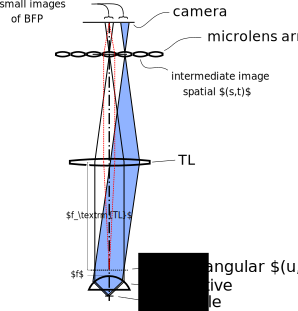
\includegraphics[width=7cm]{microlens-levoy-sketch} %FIXME redraw
  \input{microlens-levoy-sketch.eps_tex}
  \caption{Schematic of microlenses in intermediate image plane
    \citep[inspired from][]{Levoy2006}}
  \label{fig:microlens-levoy-sketch}
\end{figure}

A microlens array is placed behind the intermediate image plane (see
\figref{fig:microlens-levoy-sketch}). The light that illuminates one
microlens corresponds to one spot in the focal plane of the
sample. The camera is positioned in the focal plane of the microlenses
and captures an image of the back focal plane behind each microlens
(see dashed ray bundle in \figref{fig:microlens-levoy-sketch}).

The camera captures the four dimensional light field, leaving the
specimen with spatial coordinates $(s,t)$ and angular coordinates
$(u,v)$. This data enables computational viewpoint shifting,
refocusing, extended depth of field and aberration correction of the
detected fluorescence emission.


\begin{figure}[!hbt]
  \centering
  \input{microlens-levoy-sketch_2.eps_tex}
  \caption{Construction of an out-of-focus ray bundle through the
    light field microscope. In order to improve the readability of the
    drawing, the magnification in the microscope was set to $1:1$
    (focal lengths of tube lens and objective are equal). An on-axis
    sample point originating from below the focal plane of the
    objective is imaged onto an on-axis point between the tube lens
    and the microlens array. Three of the microlenses re-image this
    on-axis image point into three points behind the plane of the
    camera.}
  \label{fig:microlens-levoy-sketch_2}
\end{figure}

\figref{fig:microlens-levoy-sketch_2} shows a bundle of rays
originating from an out-of-focus point. Each of the microlenses that
are hit by the circle of confusion, re-image a fraction of the angular
range into a small image.  This process is crucial because a lot of
the original image information is lost here. The intensities from the
sub-images on the camera can't later be recombined in order to, say,
recover a high resolution image of the defocused point
\citetext{priv.\ comm.\ R.~Heintzmann}.

Additionally the light field microscope doesn't utilize the full
resolution of high-NA objectives. This will prevent the use of this
technique in its current form in the detection path of microscopes.

However, the same idea can be applied in the excitation path
\citep{Levoy2009}. For illumination purposes, lower resolution will
often suffice. The light-field technique allows unique control of
excitation light intensity and angles at each point of the sample
plane.

\nomenclature{TL}{tube lens}
\subsection{Temporal focusing}
\begin{figure}[!hbt]
  \centering
  %\bild{oron} 
  \input{temporal-focus-sketch.eps_tex}
  \caption{Schematic of temporal focusing \citep[inspired
    from][]{Oron2005}. A grating in the intermediate image plane
    separates the pulse into its spectral components. The out-of-focus
    areas of the specimen are illuminated with a longer pulse. Only in
    the focal plane, all spectral components interfere coherently and
    form a short intensive pulse.}
  \label{fig:oron}
\end{figure}
The axial extent of ultra-short laser pulses can be as thin as a few
microns. A parallel beam can be split into different spectral
components by a grating in the intermediate image plane
\citep{Oron2005}. The tube lens focuses the diffraction pattern into a
line in the back focal plane of the objective.

The objective, which has to be corrected for chromatic aberration and
dispersion, then focuses all the beams onto the focal plane. Different
spectral components arrive in the focal plane at the same time. The
out-of-focus points see an extended illumination. For a high NA
objective, a pulse duration of $\tau=\unit[20]{fs}$ results in slice
of $z\approx\tau c/2\approx\unit[3]{\mu m}$ thickness around the
focus, where the beam has significant intensity.

Using this technique it is possible to build a wide field 2-photon
microscope. That only excites fluorophores within the focal plane. The
technique can be further improved by spatially modulating the beam in
the intermediate image plane for CLEM like performance. This technique
has been implemented in the TF-GPC approach and will be discussed in
the next section.

\subsection{Phase modulation}
\subsubsection{Digital holography}
\begin{figure}[!hbt]
  \centering
  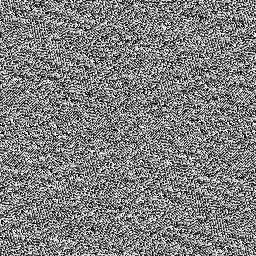
\includegraphics{myholo}\quad
  \input{phase-holo_my.eps_tex} 
  \caption{Schematic of spatial illumination by phase holography. A
    phase-only SLM displays a hologram in the plane $P'$ which is
    conjugated to the back focal plane $P$ of the objective
    \citetext{inspired by slide from V. Emiliani}.}
  \label{fig:phase-holo}
\end{figure}
Certain types of liquid crystal spatial light modulators can be used
to modify the phase of light. When such a device is placed into the
back focal plane of a lens, it is possible to control the light
distribution in its front focal plane. An iterative algorithm
(iterative Fourier transform algorithm, IFTA) can be used to establish
a phase image on the liquid crystal display that will result in an
intensity distribution in front of the lens.

\nomenclature{IFTA}{Iterative Fourier transform algorithm}

This approach has been used to excite a two-dimensional pattern in the
specimen \citep{Lutz2008,Zahid2010} and is advantageous especially for
cases where only small parts of the specimen ought to be
illuminated. As opposed to conventional intensity spatial light
modulators, the light can be redirected from dark areas into the
bright areas.

% single photon 405nm uncaging, ifta,
% spherical wave approximation
There is also a limited possibility to create three-dimensional
patterns, e.g.\ several points below, in and above the focal plane by
displaying Fresnel zone planes.  For illumination, usually a laser
with non-zero interference length is employed. However, this
illumination contains an unwanted ``speckle'' pattern in the form of
noisy non-uniformities. To a certain extent, the contrast of the
speckle pattern can be reduced by controlling spatial and temporal
coherence of the illumination (sweeping the frequency of the laser or
changing illumination direction while the detector is integrating).

Holographic control can be used with 2-photon excitation as well
\citep{Nikolenko2008}, % two photon
but this exacerbates the effect of speckles.
\subsubsection{Generalized phase contrast (GPC)}
\begin{figure}[!hbt]
  \centering
  \includegraphics[width=14cm]{phase} % FIXME redraw
  \caption{Schematic of generalized phase contrast
    \citep[from][]{Rodrigo2008}.}
  \label{fig:phase}
\end{figure}
A phase contrast microscope objective \todo{modified ?} can be used to
convert a phase image from the intermediate image plane into an
intensity image in the specimen \citep{Rodrigo2008}\todo{read more of
  this}. Compared to digital holography, hardly any computation is
necessary. Yet, the phase spatial light modulator allows to
concentrate a lot of light even on a small region of the specimen as
opposed to other techniques, which involve intensity modulation and
lose all the light of dark areas by sending it into a beam block or
something similar.

The generalized phase contrast method is suitable even with spatially
incoherent illumination\todo{slightly ?}.
\subsubsection{Generalized phase contrast and temporal focusing (TF-GPC)}
The combination of generalized phase contrast and temporal focusing
allows spatially controlled illumination of in-focus areas
\citep{Papagiakoumou2010}. Usage of a phase spatial light modulator
results in high light efficiency compared to intensity modulation.
Splitting and recombination of the spectral components of the pulse
reduce speckle noise considerably.
\begin{figure}[!hbt]
  \centering
  \includegraphics[width=11cm]{tf-gpc} 
  \caption{Schematic of phase contrast with temporal focusing (TF-GPC)
    \citep[from][]{Papagiakoumou2010}, PCF is a phase contrast filter.}
  \label{fig:tf-gpc}
\end{figure}
\nomenclature{PCF}{Phase contrast filter}

%%% Local Variables: 
%%% mode: latex
%%% TeX-master: "kielhorn_memi"
%%% End: 
